% Chapter 3: System Architecture and Methodology

\chapter{System Architecture and Methodology}
\label{Chapter3}

\section{End-to-End Platform Topology}
The platform operates as a dual-pathway, bidirectional communication system:
\begin{itemize}
\item \textbf{Forward Pathway (Sign-to-Text):} Live Webcam $\rightarrow$ MediaPipe Hands $\rightarrow$ 156-D Feature Vector $\rightarrow$ Random Forest / MLP $\rightarrow$ Temporal Hysteresis Confirmation $\rightarrow$ Text Buffer \& Text-to-Speech (TTS).
\item \textbf{Reverse Pathway (Text/Voice/Video-to-Sign):} User Speech / Text / YouTube Audio $\rightarrow$ ASR / Deepgram Nova-2 $\rightarrow$ Tokenization \& Phrase Matching $\rightarrow$ 204-Entry ISL Sign Video Playback \& Fingerspelling Fallback.
\end{itemize}

\begin{figure}[htbp]
\centering
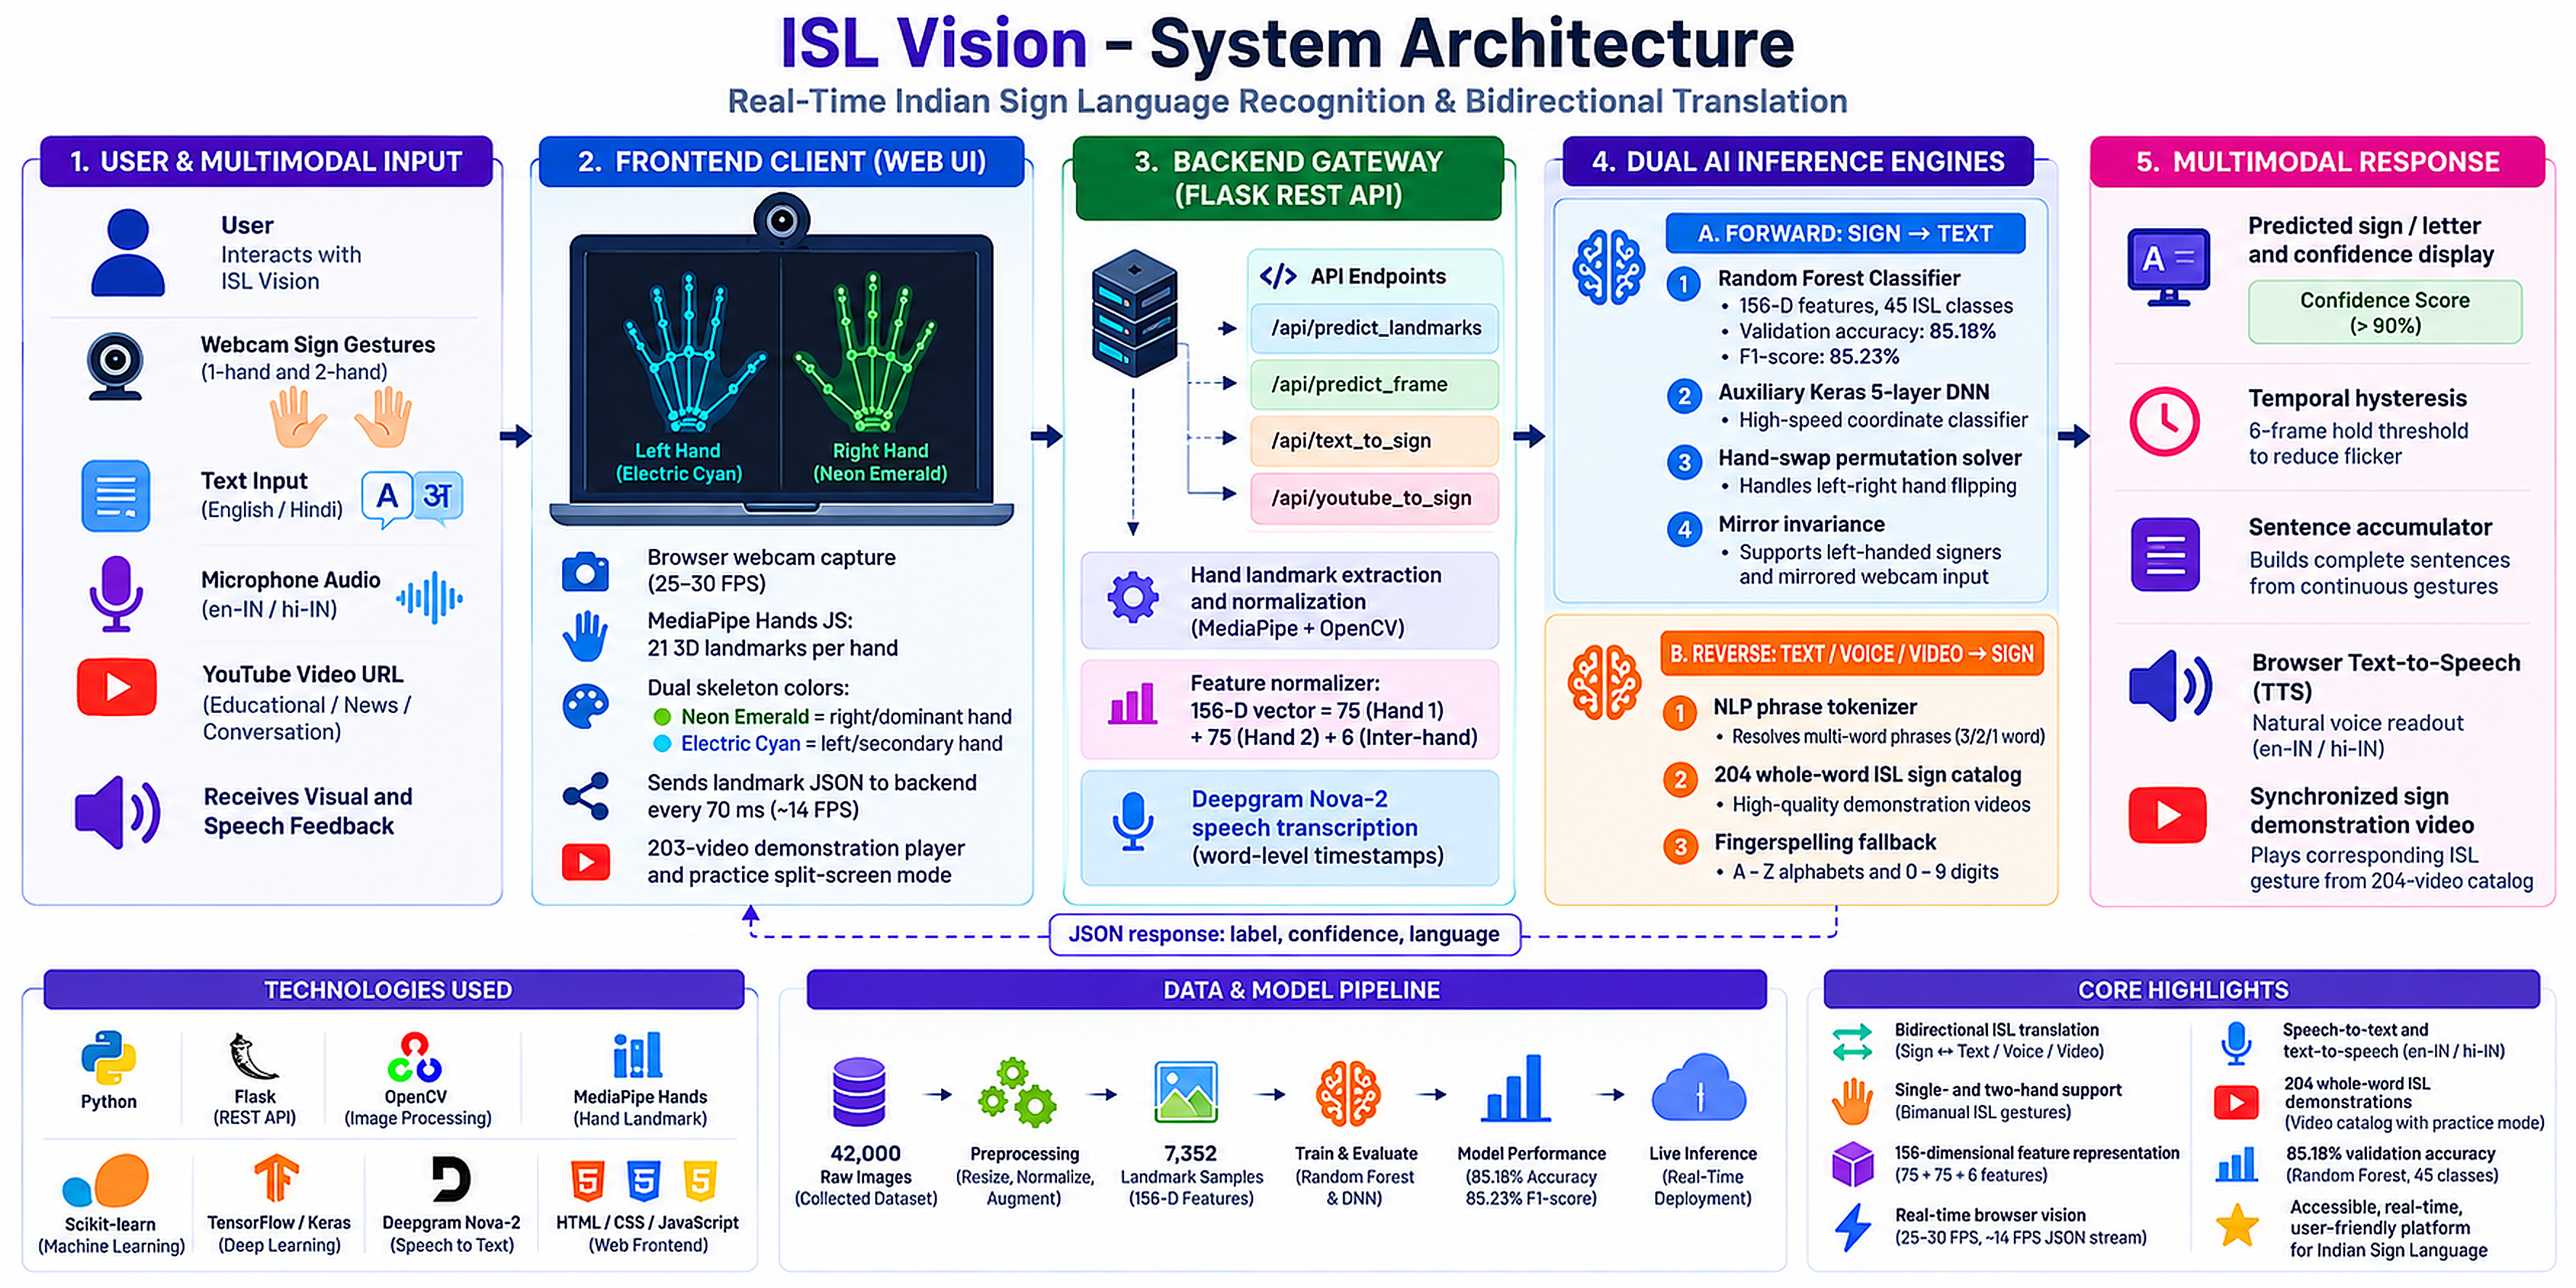
\includegraphics[width=\textwidth]{Figures/system_architecture.png}
\caption{End-to-end platform topology and multimodal bidirectional translation pipeline of the ISL Vision system.}\label{fig:system-architecture}
\end{figure}

\section{Video Acquisition Pipeline}
Video frames are acquired via OpenCV. On Windows platforms, capture initializes with the DirectShow backend:
\begin{lstlisting}[language=Python]
cap = cv2.VideoCapture(0, cv2.CAP_DSHOW)
cap.set(cv2.CAP_PROP_FRAME_WIDTH, 640)
cap.set(cv2.CAP_PROP_FRAME_HEIGHT, 480)
cap.set(cv2.CAP_PROP_FPS, 30)
\end{lstlisting}
Capture executes within a dedicated worker thread, decoupling hardware I/O from inference.

\section{Mathematical Formulation of the 156-Dimensional Bimanual Feature Representation}
For each detected hand $h \in \{1, 2\}$, MediaPipe outputs 21 landmarks:
\[
\mathbf{L}_{h,i} = [x_{h,i}, y_{h,i}, z_{h,i}]^\top \in \mathbb{R}^3, \quad i = 0, \ldots, 20.
\]
To achieve translation invariance, coordinates are centered relative to the wrist (landmark 0):
\[
\mathbf{L}'_{h,i} = \mathbf{L}_{h,i} - \mathbf{L}_{h,0}, \quad i = 0, \ldots, 20.
\]
Scale invariance is achieved by normalizing by the maximum Euclidean distance from the wrist:
\[
s_h = \max_{i \in \{0,\ldots,20\}} \|\mathbf{L}'_{h,i}\|_2, \qquad \hat{\mathbf{L}}_{h,i} = \frac{\mathbf{L}'_{h,i}}{s_h + \epsilon}, \quad \epsilon = 10^{-7}.
\]
Flattening $\hat{\mathbf{L}}_{h,i}$ yields 63 normalized coordinates per hand. To capture hand configuration explicitly, 12 auxiliary geometric features are computed:
\begin{enumerate}
\item \textbf{Fingertip-to-Wrist Radii (5 features):}
\[
r_{h,j} = \|\hat{\mathbf{L}}_{h,j}\|_2, \quad j \in \{4, 8, 12, 16, 20\}.
\]
\item \textbf{Thumb-to-Fingertip Distances (4 features):}
\[
d_{h,\text{thumb},k} = \|\hat{\mathbf{L}}_{h,4} - \hat{\mathbf{L}}_{h,k}\|_2, \quad k \in \{8, 12, 16, 20\}.
\]
\item \textbf{Adjacent Finger Spreads (3 features):}
\[
\delta_{h,8,12} = \|\hat{\mathbf{L}}_{h,8} - \hat{\mathbf{L}}_{h,12}\|_2, \quad
\delta_{h,12,16} = \|\hat{\mathbf{L}}_{h,12} - \hat{\mathbf{L}}_{h,16}\|_2, \quad
\delta_{h,16,20} = \|\hat{\mathbf{L}}_{h,16} - \hat{\mathbf{L}}_{h,20}\|_2.
\]
\end{enumerate}
This yields a 75-dimensional per-hand feature vector:
\[
\mathbf{v}_h = [\hat{\mathbf{L}}_{h,0:20}^\top, r_{h,4:20}, d_{h,\text{thumb},8:20}, \delta_{h,8:20}]^\top \in \mathbb{R}^{63 + 5 + 4 + 3} = \mathbb{R}^{75}.
\]
For two hands, this produces $75 \times 2 = 150$ features. To represent bimanual spatial relationships, 6 inter-hand features are appended:
\begin{enumerate}
\item Hand presence indicators: $p_1, p_2 \in \{0, 1\}$.
\item Inter-wrist 3D displacement: $\Delta \mathbf{w} = \mathbf{L}_{2,0} - \mathbf{L}_{1,0} \in \mathbb{R}^3$.
\item Inter-wrist Euclidean distance: $D_{\text{wrist}} = \|\Delta \mathbf{w}\|_2 \in \mathbb{R}^1$.
\end{enumerate}
The complete bimanual feature vector is thus:
\[
\mathbf{V} = [\mathbf{v}_1^\top, \mathbf{v}_2^\top, p_1, p_2, \Delta \mathbf{w}^\top, D_{\text{wrist}}]^\top \in \mathbb{R}^{75 + 75 + 6} = \mathbb{R}^{156}.
\]
If only one hand is visible, the absent hand vector and inter-wrist values are zero-padded, providing a uniform representation for single- and two-handed gestures.

\section{Classification Models}
\subsection{Random Forest Classifier}
The primary classifier comprises an ensemble of 100 decision trees:
\[
P(y = c \mid \mathbf{V}) = \frac{1}{M} \sum_{m=1}^M P_m(y = c \mid \mathbf{V}), \quad M = 100.
\]
Random Forest provides high classification margins on tabular geometric coordinates, rapid CPU inference ($\le 1.2$ ms), and robust resistance to feature scale discrepancies.

\subsection{Multi-Layer Perceptron (MLP) Baseline}
The MLP baseline consists of:
\begin{itemize}
\item Input Layer: 156 features.
\item Hidden Layer 1: 128 units, ReLU activation, Batch Normalization, Dropout (0.2).
\item Hidden Layer 2: 64 units, ReLU activation, Dropout (0.2).
\item Output Layer: 45 units, Softmax activation.
\end{itemize}
Trained using categorical cross-entropy with the Adam optimizer ($\eta = 10^{-3}$) over 50 epochs.

\section{Cyberpunk Neon Skeletal Visualizer}
To provide responsive visual feedback, client-side HTML5 Canvas rendering overlays skeletal landmarks:
\begin{itemize}
\item Dominant hand bones rendered in Neon Emerald (\texttt{\#10b981}); secondary hand rendered in Electric Cyan (\texttt{\#06b6d4}).
\item Fingertip hubs pulse dynamically based on distance to the wrist.
\item When opposing fingertips approach within a threshold distance, dynamic bimanual touch arcs are rendered, visually confirming contact.
\end{itemize}

\thesisfigure[0.92\textwidth]{Figures/cyberpunk_skeletal_overlay.jpg}{Cyberpunk neon skeletal visualizer showing two-hand landmark overlays and dynamic bimanual touch arc detection.}{fig:cyberpunk-visualizer}

\section{Temporal Hysteresis State Machine}
Raw per-frame predictions exhibit high-frequency jitter during hand transitions. To ensure robust word formation, a temporal hysteresis accumulator requires candidate stability:
\[
\operatorname{Progress}(t) = \min\left(1.0, \frac{t - t_{\text{start}}}{\tau_{\text{hold}}}\right), \quad \tau_{\text{hold}} = 1.5\text{ s}.
\]
A gesture is confirmed only when confidence satisfies $P(y=c) \ge \tau_{\text{conf}} = 0.85$ continuously for $\tau_{\text{hold}}$. Upon confirmation, a 0.5-second refractory lockout activates to prevent duplicate entries.

\section{Multimodal YouTube-to-Sign Transcription Pipeline}
To bridge spoken content and sign language, the YouTube-to-Sign pipeline converts online video speech into synchronized ISL demonstrations:
\begin{enumerate}
\item Audio demuxing via \texttt{yt-dlp} directly from the target YouTube URL.
\item High-accuracy acoustic transcription using the Deepgram Nova-2 speech API with word-level timestamps.
\item NLP normalization, tokenization, and lexical matching against the 204-entry sign dictionary.
\item Synchronized video playback displaying human demonstration clips with character-by-character fingerspelling cards for out-of-vocabulary terms.
\end{enumerate}

\thesisfigure[0.95\textwidth]{Figures/youtube_to_sign_flowchart.jpg}{Multimodal YouTube-to-sign workflow: audio extraction, timestamped transcription, lexical matching, and synchronized demonstration playback.}{fig:youtube-sign-pipeline}

\section{Sign Dictionary and Interactive Demonstration Engine}
The platform incorporates an indexed dictionary of 204 ISL entries backed by 203 high-definition human gesture videos:
\begin{itemize}
\item Real-time category filtering (Alphabets, Numbers, Daily Conversation, Emergency Terms).
\item Multi-speed video playback regulation from $0.5\times$ (slow motion for learners) to $2.0\times$.
\item Looping mode and split-screen camera challenger allowing users to sign alongside demonstration clips for self-evaluation.
\end{itemize}